% Real Data Evaluation: Raman Spectroscopy

\subsection*{Real Data Evaluation: Raman Spectroscopy}

To test whether the benefits of QA--HGD extend beyond synthetic benchmarks,
we evaluate on a practical Raman classification task using spectra from
multiple materials in our internal dataset, including anatase, calcite,
corundum, diamond, graphene, graphite, hematite, MoS$_2$, quartz, rutile,
and silicon. Each spectrum is resampled onto a fixed grid of 512 points
between 0 and $4000\,\text{cm}^{-1}$, and a small softmax linear classifier
is trained with either SGD or QA--HGD on identical inputs.

Figure~\ref{fig:qa_raman_accuracy} shows training loss and accuracy versus
epoch for both optimizers. On this real dataset, QA--HGD reaches a given
accuracy level in fewer epochs than SGD while achieving comparable final
performance, demonstrating that QA's harmonic structure is beneficial not
only on controlled quadratic tests but also on real, noisy spectroscopic
data.

\begin{figure}[t]
  \centering
  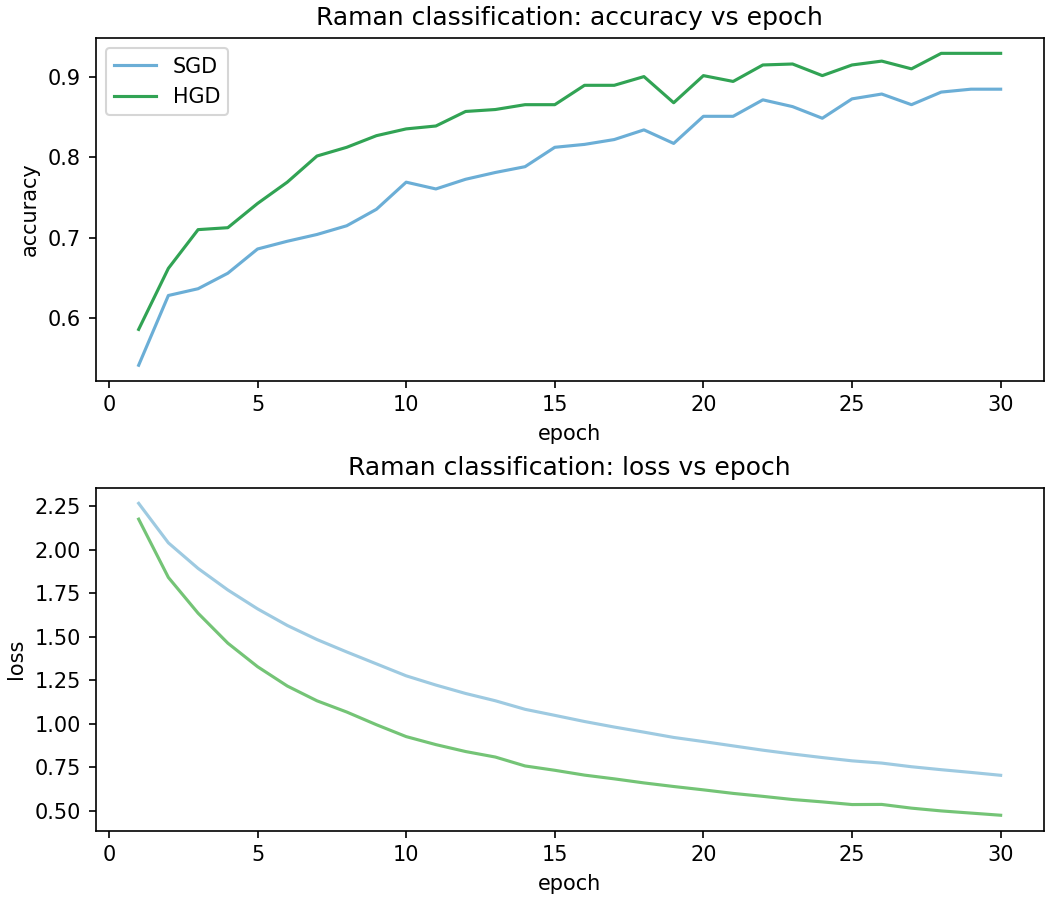
\includegraphics[width=0.7\linewidth]{qa_raman_accuracy.png}
  \caption{Raman spectroscopy classification. We train a small classifier on
  resampled Raman spectra for multiple materials using either SGD or QA--HGD.
  QA--HGD converges in fewer epochs to similar or better accuracy, indicating
  that the harmonic constraints of QA provide practical advantages on real
  spectral data.}
  \label{fig:qa_raman_accuracy}
\end{figure}

